\documentclass[11pt,a4paper]{article}
\usepackage[margin=21mm,headheight=15pt]{geometry}
\usepackage[T1]{fontenc}
\usepackage[utf8]{inputenc}
\usepackage{mathpazo,amsmath,amssymb,graphicx,booktabs,enumitem,microtype,float}
\usepackage[font=normalsize,labelfont=bf]{caption}
\usepackage[hidelinks]{hyperref}
\usepackage{fancyhdr}
\linespread{1.025}
\setlength{\parindent}{0pt}
\setlength{\parskip}{5pt}
\setlength{\tabcolsep}{6pt}
\renewcommand{\arraystretch}{1.12}
\setlist{nosep,leftmargin=*}
\pagestyle{fancy}\fancyhf{}
\fancyhead[L]{Team 87: Lebmar}\fancyhead[R]{2026 MCM Senior Group, Problem A}
\fancyfoot[C]{\thepage}
\graphicspath{{images/}}
\newcommand{\BaseGrowth}{3.38}
\newcommand{\PolicyGrowth}{3.66}
\newcommand{\BaseLoss}{39.52}
\newcommand{\PolicyLoss}{43.44}
\newcommand{\PolicyTrade}{35.5}
\newcommand{\PolicyLaterTrade}{33.28}
\newcommand{\PolicyReview}{48.3}
\newcommand{\FeeReduction}{46.2}
\newcommand{\GrowthDifference}{0.282}
\newcommand{\GrowthDifferenceLow}{0.026}
\newcommand{\GrowthDifferenceHigh}{0.758}
\newcommand{\LossDifference}{3.92}
\newcommand{\LossDifferenceLow}{-2.18}
\newcommand{\LossDifferenceHigh}{10.95}
\newcommand{\E}{\mathbb{E}}
\begin{document}
\begin{center}
{\Large\bfseries SafeInvest: Suitability, Cost-Aware Rebalancing,\\[3pt]
and the Limits of Automation}\par
\vspace{7pt}
{\large Chengxuan YUAN}\par
Team Lebmar, No. 87 \qquad 17 October 2026
\end{center}

\section*{Executive summary}
SafeInvest must make suitable, explainable investment decisions without
pretending that automation can guarantee a customer's loss tolerance. We build
a transparent three-asset catalogue, an empirical suitability screen, and a
sequential policy that trades only when estimated net benefit exceeds an
declared conservatism margin. A distinct review state pauses trading while preserving
all subsequent investment outcomes in the evaluation.

Our frozen targets, in equity/bond/bill order, are Conservative
15/5/80, Balanced 45/10/45, and Growth 90/5/5 percent. They are selected on
development data under declared risk preferences, not chosen to force the five
customers into expected labels. The frozen onboarding rule refers A and D,
assigns B and E to Conservative, and assigns C to Balanced.
The last assignment is borderline and is not validated as a reliable automatic
recommendation: its loss-exceedance rate rises from 12/120 in development to
10/60 in the final scenarios. C therefore warrants human confirmation before
unattended deployment; we retain, rather than retrospectively rewrite, the
frozen rule and its measured outcomes.

In the 60 final 30-year scenarios, the selected fixed-target, cost-gated policy
with review has median real annual growth of \PolicyGrowth\%, compared with
\BaseGrowth\% for annual equal-weight rebalancing. It trades in
\PolicyTrade\% of reviews and incurs \FeeReduction\% less mean cumulative
fee expenditure. However, its 90th-percentile maximum real drawdown is
\PolicyLoss\%, versus \BaseLoss\% for the benchmark. This is a growth--risk
trade-off, not comprehensive superiority.

Bounded automatic target updates lower some drawdown estimates but reduce
median growth. Their incremental utility interval includes zero in both
architecture validation and final evaluation. We therefore keep the frozen
fixed-target policy and do not recommend automatic target updates on this
evidence. Review is a governance safeguard, not an effective stop-loss:
\PolicyReview\% of final paths enter review, and losses can continue.

\textbf{What is established.} Financial identities and causal timing pass
automated tests; all outcomes remain in the sample, including review periods;
source, data and configuration hashes tie final results to a frozen model.
Cost sensitivity preserves the main qualitative trade-off.

\textbf{What is not established.} Neither real-world suitability, a guaranteed
loss ceiling, reliable market prediction, nor universal policy dominance is
established by 180 synthetic annual scenarios. We treat the failure to validate
C's borderline assignment as an important result of a trustworthy system.

\newpage
\section{Accounting and purchasing-power risk}
Each scenario begins with 100 units in bills. There are no subsequent deposits
or withdrawals, short sales, leverage, taxes, other charges or terminal
liquidation. At the beginning of year $t$, a decision sees only that scenario's
observations through $t-1$. Returns for year $t$ are applied after any trade and
fee. All three assets are observed jointly with inflation.

Let $x_i$ be pre-trade nominal asset values and $V=\sum_i x_i$. For a target
$w_i\geq0$, $\sum_iw_i=1$, we explicitly adopt a fee-after allocation convention.
Money entering destination assets is charged once; sale proceeds also fund the
fee. Thus, with $c=0.0025$,
\begin{equation}
 C=c\sum_i[(V-C)w_i-x_i]_+,\qquad x_i'=(V-C)w_i.
\end{equation}
This scalar, piecewise-linear equation is solved exactly over active
destination assets. It ensures $\sum_i x_i'=V-C$. Transferring an actual 20
units costs 0.05. A 20\% \emph{fee-after target} is slightly different because
the investable wealth has fallen. Keeping current holdings costs zero; initial
allocation uses the same equation. This payment convention is a declared
implementation choice where the problem does not specify the funding asset.

With observed nominal returns $r_{i,t}$,
\begin{equation}
 V_t=\sum_i x'_{i,t}(1+r_{i,t}),\quad
 I_t=\prod_{u=1}^{t}(1+\pi_u),\quad R_t=V_t/I_t,\quad R_0=100.
\end{equation}
Define annual net real returns $z_t=R_t/R_{t-1}-1$. For horizon $H$ we report
\begin{align}
 G_H&=(R_H/100)^{1/H}-1, &
 \sigma_H&=\operatorname{sd}(z_1,\ldots,z_H),\\
 D_H&=\max_{0\leq t\leq H}\left(1-\frac{R_t}{\max_{0\leq u\leq t}R_u}\right).
\end{align}
Growth is actual purchasing-power growth after fees. Standard deviation
describes ordinary fluctuations; maximum drawdown describes a large
peak-to-trough loss, with larger values meaning greater loss. Including $R_0$
prevents omission of first-year allocation costs. Relative real drawdown is our
explicit definition; we do not import a Brownian market assumption from the
drawdown literature [6].

All drawdowns use annual observations. A fee reduces the subsequent net wealth,
but we do not add a fee-only intrayear observation to the drawdown series. This
keeps forecasting and reporting consistent. Actual intrayear drawdowns may be
larger and cannot be recovered from the supplied data.

For each scenario, metrics are calculated first and then summarized across
scenarios. The P90 of $D_H$ is therefore the 90th percentile of scenario-level
maximum drawdowns, not a percentile of annual returns. The bill proxy is not
real-risk-free: inflation can reduce its purchasing power. This prevents
equating a high bill allocation with guaranteed preservation.

\newpage
\section{A product catalogue and a suitability process}
We consider 5-percentage-point simplex weights, require at least 5\% in each
asset, and add the exact equal-weight target. This gives 172 candidates. Fixed
targets are annually restored during catalogue fitting, including all costs.
The catalogue uses the declared objective
\begin{equation}
 J_H(w;\lambda)=\E[\log(R_H(w)/100)]-\lambda\E[D_H(w)].
\end{equation}
At $H=30$, coefficients $\lambda=10,4,1$ express increasingly growth-oriented
preferences. They are policy assumptions, not customer parameters identified
from three questionnaire fields. Bill floors are 30\%, 10\%, and 5\%,
respectively. The original 1--80 fit and final 1--120 refit use the same rule.
The Balanced refit changes from 60/15/25 to 45/10/45, illustrating estimation
sensitivity; the neighbourhood in the fitting grid is comparatively flat.

\begin{center}
\begin{tabular}{lrrrr}
\toprule
Product & Equity & Bond & Bill & $\lambda$\\\midrule
Conservative & 15\% & 5\% & 80\% & 10\\
Balanced & 45\% & 10\% & 45\% & 4\\
Growth & 90\% & 5\% & 5\% & 1\\\bottomrule
\end{tabular}
\end{center}
Conservative and Growth restore their fixed targets annually. Balanced uses
the selected cost-aware policy. The names describe relative product risk,
not guaranteed loss ranges or compulsory assignments.

For customer $j$, we use exactly $H_j=5,15,30,25,6$ years for A--E. A product
passes our empirical loss screen if
\begin{equation}
 \widehat p_j=\frac{1}{120}\sum_{s=1}^{120}
 \mathbf1\{D_{s,H_j}>L_j\}\leq0.10.
\end{equation}
Bill floors for high/medium/low liquidity are 30/10/0 percent. Among passing
products, choose the highest development median real CAGR; if none pass, refer.
These are transparent service policies, not organizer-imposed thresholds or
90\% safety guarantees. No withdrawal sufficiency is tested because the
experiment has no withdrawals. Wilson intervals accompany exceedance rates.

\begin{center}
\begin{tabular}{clrrl}
\toprule
Client & Frozen action & $H$ & Tolerance & Explanation\\\midrule
A & Human review & 5 & 10\% & No product passes loss screen\\
B & Conservative & 15 & 25\% & 2/120 exceedances\\
C & Balanced & 30 & 40\% & 12/120; exactly at cutoff\\
D & Human review & 25 & 15\% & Long horizon does not offset low tolerance\\
E & Conservative & 6 & 35\% & Both liquid choices pass; higher fitted growth\\\bottomrule
\end{tabular}
\end{center}
For A and D this is a statement about the available catalogue, not proof that
every possible investment rule is unsuitable. In fitting-only checks, no
fixed grid target met their strict screen under the stated liquidity floor.
Changing the cutoff to 5\% moves C to Conservative; at 20\%, A becomes
Conservative and B Balanced. These differences expose policy sensitivity.

\newpage
\section{Cost-aware annual decisions and human review}
We use four unguarded strategies to separate effects and two guarded variants:
\begin{center}
\begin{tabular}{ll}
\toprule
Rule & Definition\\\midrule
S0 & Equal-weight target, restore annually (required baseline)\\
S1 & Chosen Balanced target, restore annually\\
S2 & Same fixed target, trade only after net-benefit test\\
S3 & Same executor, allow bounded target changes\\
S2+R, S3+R & Add the same explicit review/pending rule\\\bottomrule
\end{tabular}
\end{center}
S1--S0 separates target choice; S2--S1 execution; S3--S2 target updates.
Guarded versus corresponding unguarded results measure the effect of pending
behaviour. This avoids attributing an allocation change to clever timing.

\textbf{Forecasting assumption.} From fitting scenarios only, sample 256 joint
paths by concatenating six continuous five-year blocks. Assets and inflation
stay together; random seed is 1729. At year $t$, use the remaining $H-t+1$
years of these paths. All actions share identical forecast paths. This assumes
development blocks remain representative and is not evidence of return
predictability. Conditional market timing is deliberately omitted.

\textbf{Action comparison.} Current holdings are normalized by current wealth.
For each possible action, apply its self-financing fee, project drifting
holdings without additional forecast trades, and compute
\begin{equation}
 Q_t(a)=\widehat\E[\log(R_H^a/R_{t-1})]-4\widehat\E[D_H^a].
\end{equation}
The drawdown extends the actual historical peak and already realized maximum
drawdown. The future cannot erase a past loss. The best action is taken only
if $Q_t(a)>Q_t(\mathrm{keep})+0.002$. The margin is in total utility units;
cost is already reflected in wealth and is not subtracted twice. Initially,
only bills versus the base catalogue target are compared; the dynamic
neighbourhood opens from the second review. Rejecting all actions keeps
both current holdings and the approved target unchanged.

For S3, equity targets are the original Balanced equity weight plus
$\{-0.10,-0.05,0,0.05,0.10\}$. Non-equity weights retain their original
bond/bill ratio; bill weight must remain at least 10\%. A single target change
cannot exceed 5 percentage points. Global targets therefore cannot drift
indefinitely. Actual holdings can drift beyond target bounds between trades.

\textbf{Review and pending.} In the generic Balanced experiment, an observed
real drawdown of at least 25\% triggers review at the next annual decision.
Customer-specific diagnostics instead use that customer's stated tolerance.
While review is pending, no further trading or target updates occur; returns
and all scoring continue. Without human-decision data we keep the path pending
through its remaining horizon, rather than inventing perfect human decisions.
The rule does not cap losses at the threshold. Invalid inputs also require
suspension; the input loader rejects missing or non-finite observations
rather than treating them as zero returns.

\newpage
\section{Development, validation and a frozen decision}
The organisers supply 180 independent synthetic scenarios, each with 30 annual
periods, based on selected U.S. JST Release 6 series [1--3]. Raw historical
database observations are not used. Scenarios 1--80 fit the catalogue and forecast bank;
81--120 compare fixed architectures. The fixed risk coefficients, fee rule,
0.002 utility margin, forecast specification and bounded action set are written
in the protocol. No validation parameter search is performed.

\begin{figure}[H]
\centering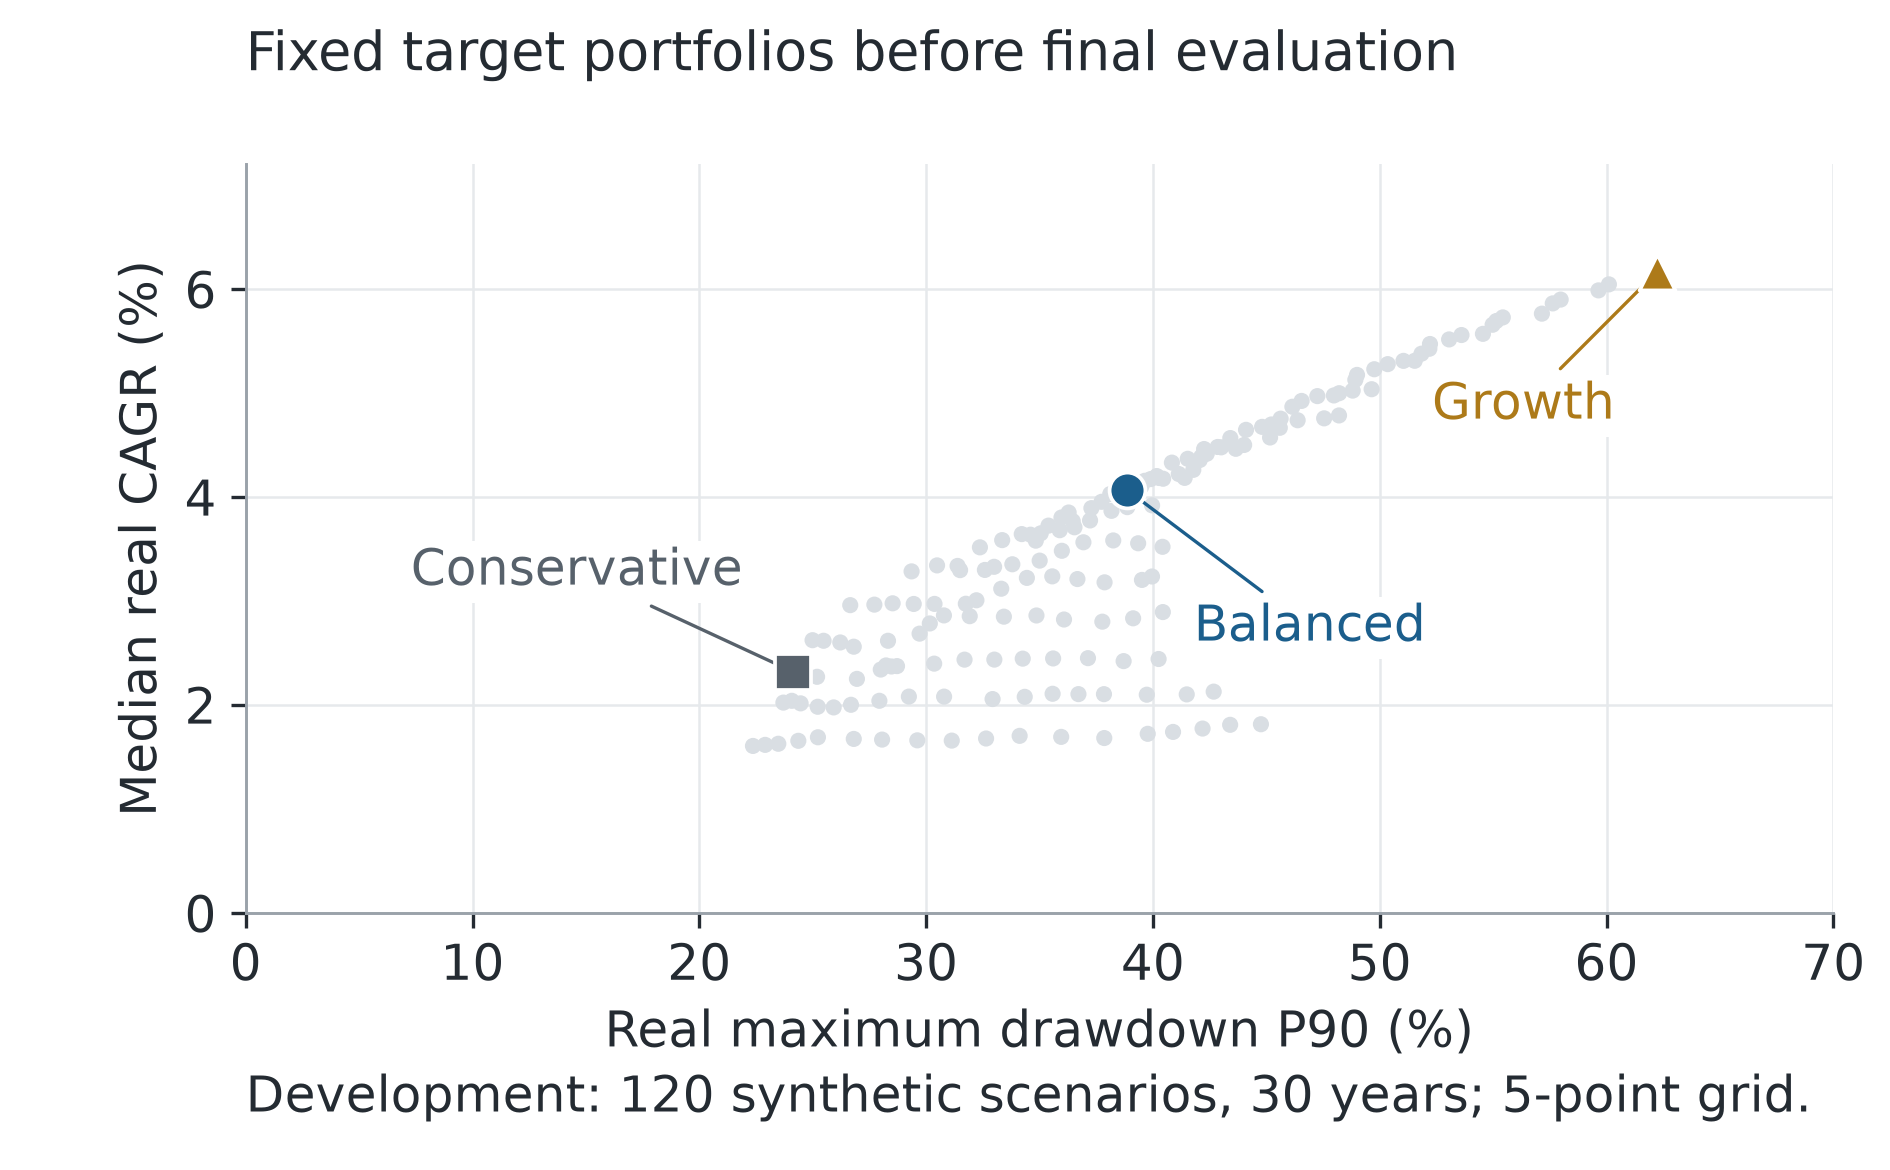
\includegraphics[width=0.94\linewidth]{01_portfolio_grid.png}
\caption{Development catalogue: growth versus large-loss risk, with the final
refitted targets marked. Synthetic contest data, scenarios 1--120. These are
fitting diagnostics, not out-of-sample performance.}
\end{figure}

The architecture rule enables S3+R only if its paired mean utility advantage
over S2+R has a positive 95\% bootstrap lower endpoint, its P90 drawdown rises
by no more than 2 percentage points, and P10 CAGR falls by no more than 0.25
percentage points. The latter two are empirical screens, not statistical
noninferiority guarantees. The 4,000 paired resamples preserve complete
scenarios and use a fixed seed.

Validation yields incremental mean utility 0.0440 with interval
$[-0.0063,0.0962]$. S3+R therefore fails the first criterion. We select S2+R,
refit weights and the forecast bank once on 1--120, and freeze the architecture,
customer assignments, sources, protocol, data and forecast hashes. The final
60 paths are then evaluated without further adjustment. Equal-weight rules
remain valuable comparators under estimation error [5]; this does not prove
equal weighting optimal in our synthetic task. Cost-aware sequential decisions
are motivated by [4], without importing a convexity or optimality claim.

\textbf{Exposure and development corrections.} Before formal development, a
source inventory printed pooled descriptive statistics over all 180 paths.
No strategy selection used them, but this is not a completely pristine blind
test. Independent review corrected initial-allocation gating and a forecast
versus annual-drawdown measurement mismatch; development was rerun before any
final policy evaluation. The 1--120 suitability estimates are refitted,
in-sample diagnostics. Final customer results audit them without rewriting
their frozen assignments. These qualifications are retained in the audit log.

\newpage
\section{Final evaluation: gains come with trade-offs}
Table 1 uses all 60 final paths, including the 100-unit starting point and
every pending-review year. Percentages are net real results; trade rate
includes initial reviews. S2+R is the frozen policy.

\begin{table}[H]\centering
\caption{Thirty-year final results, all entries in percent. $G$: real CAGR;
$D$: maximum real drawdown.}
\begin{tabular}{lrrrrr}\toprule
Rule & Median $G$ & P10 $G$ & Median $D$ & P90 $D$ & Trade rate\\\midrule
\input table_results.tex
\bottomrule\end{tabular}
\end{table}

\begin{figure}[H]\centering
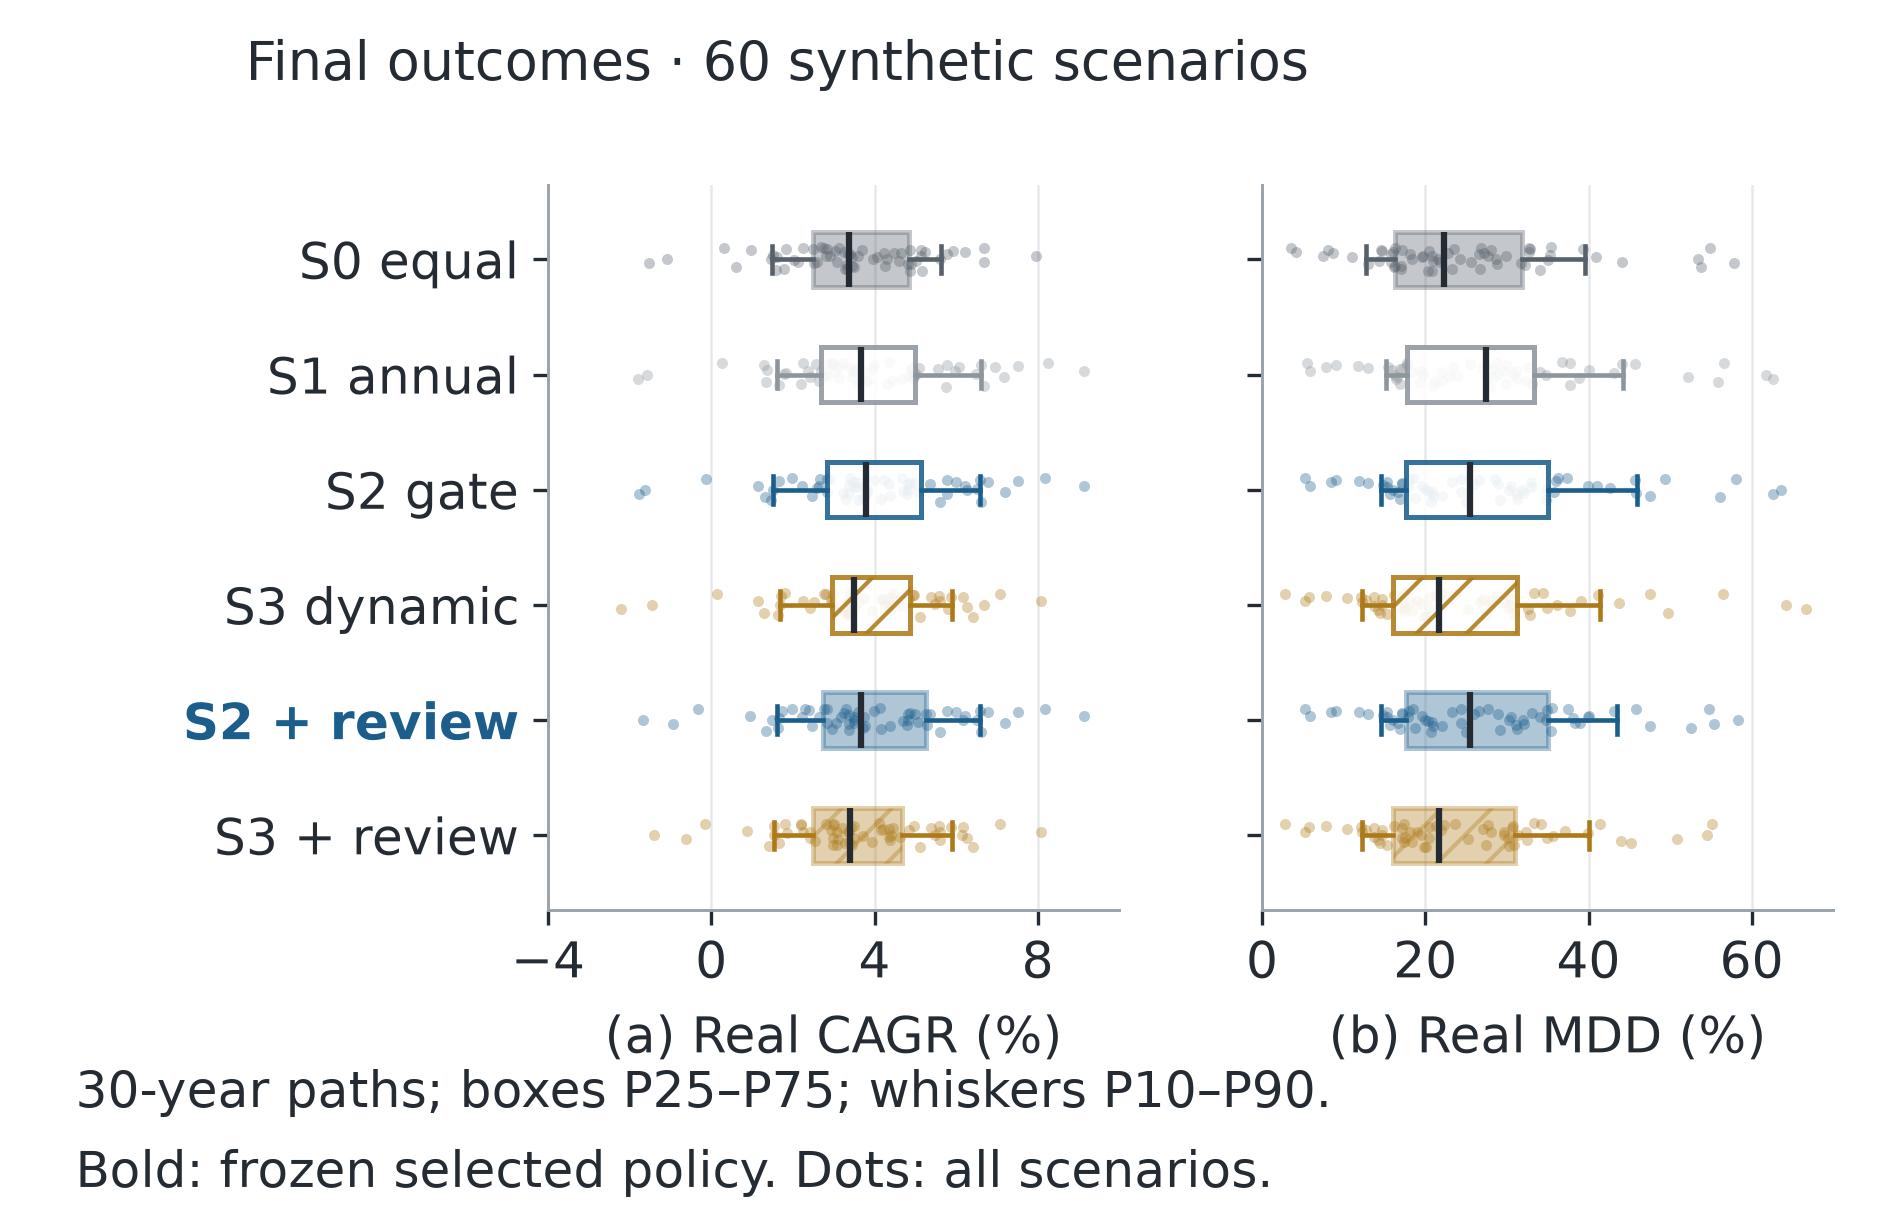
\includegraphics[width=0.94\linewidth]{02_final_distributions.png}
\caption{Final scenario distributions. Spread across scenarios is distinct
from uncertainty in a mean or quantile; displayed distribution ranges are not
confidence intervals. Synthetic contest data, $n=60$.}
\end{figure}

S2+R's median growth difference from S0 is \GrowthDifference{} percentage
points, with paired interval $[\GrowthDifferenceLow,\GrowthDifferenceHigh]$.
Its P90 drawdown difference is $+\LossDifference$ points, with interval
$[\LossDifferenceLow,\LossDifferenceHigh]$. Mean utility difference is 0.0232
with interval $[-0.0530,0.0971]$. Thus higher typical growth does not establish
an unambiguous risk-adjusted improvement. Mean fees are 0.526 versus 0.979
nominal units; this is fee expenditure, not the full compounded opportunity
cost. S2+R trades in \PolicyTrade\% of all reviews, or \PolicyLaterTrade\%
after excluding initial deployment.

S3+R versus S2+R has utility difference 0.0218, interval
$[-0.0215,0.0650]$: insufficient evidence to enable updates. Its median growth
is lower by 0.260 points while P90 drawdown is lower by 3.33 points. We keep
the validation decision; we do not switch architectures after seeing the final
table.

\newpage
\section{A severe scenario and an honest safeguard}
We preselect the final scenario with the largest S0 drawdown, rather than
choose the path where our policy wins most. This is scenario 155.

\begin{figure}[H]\centering
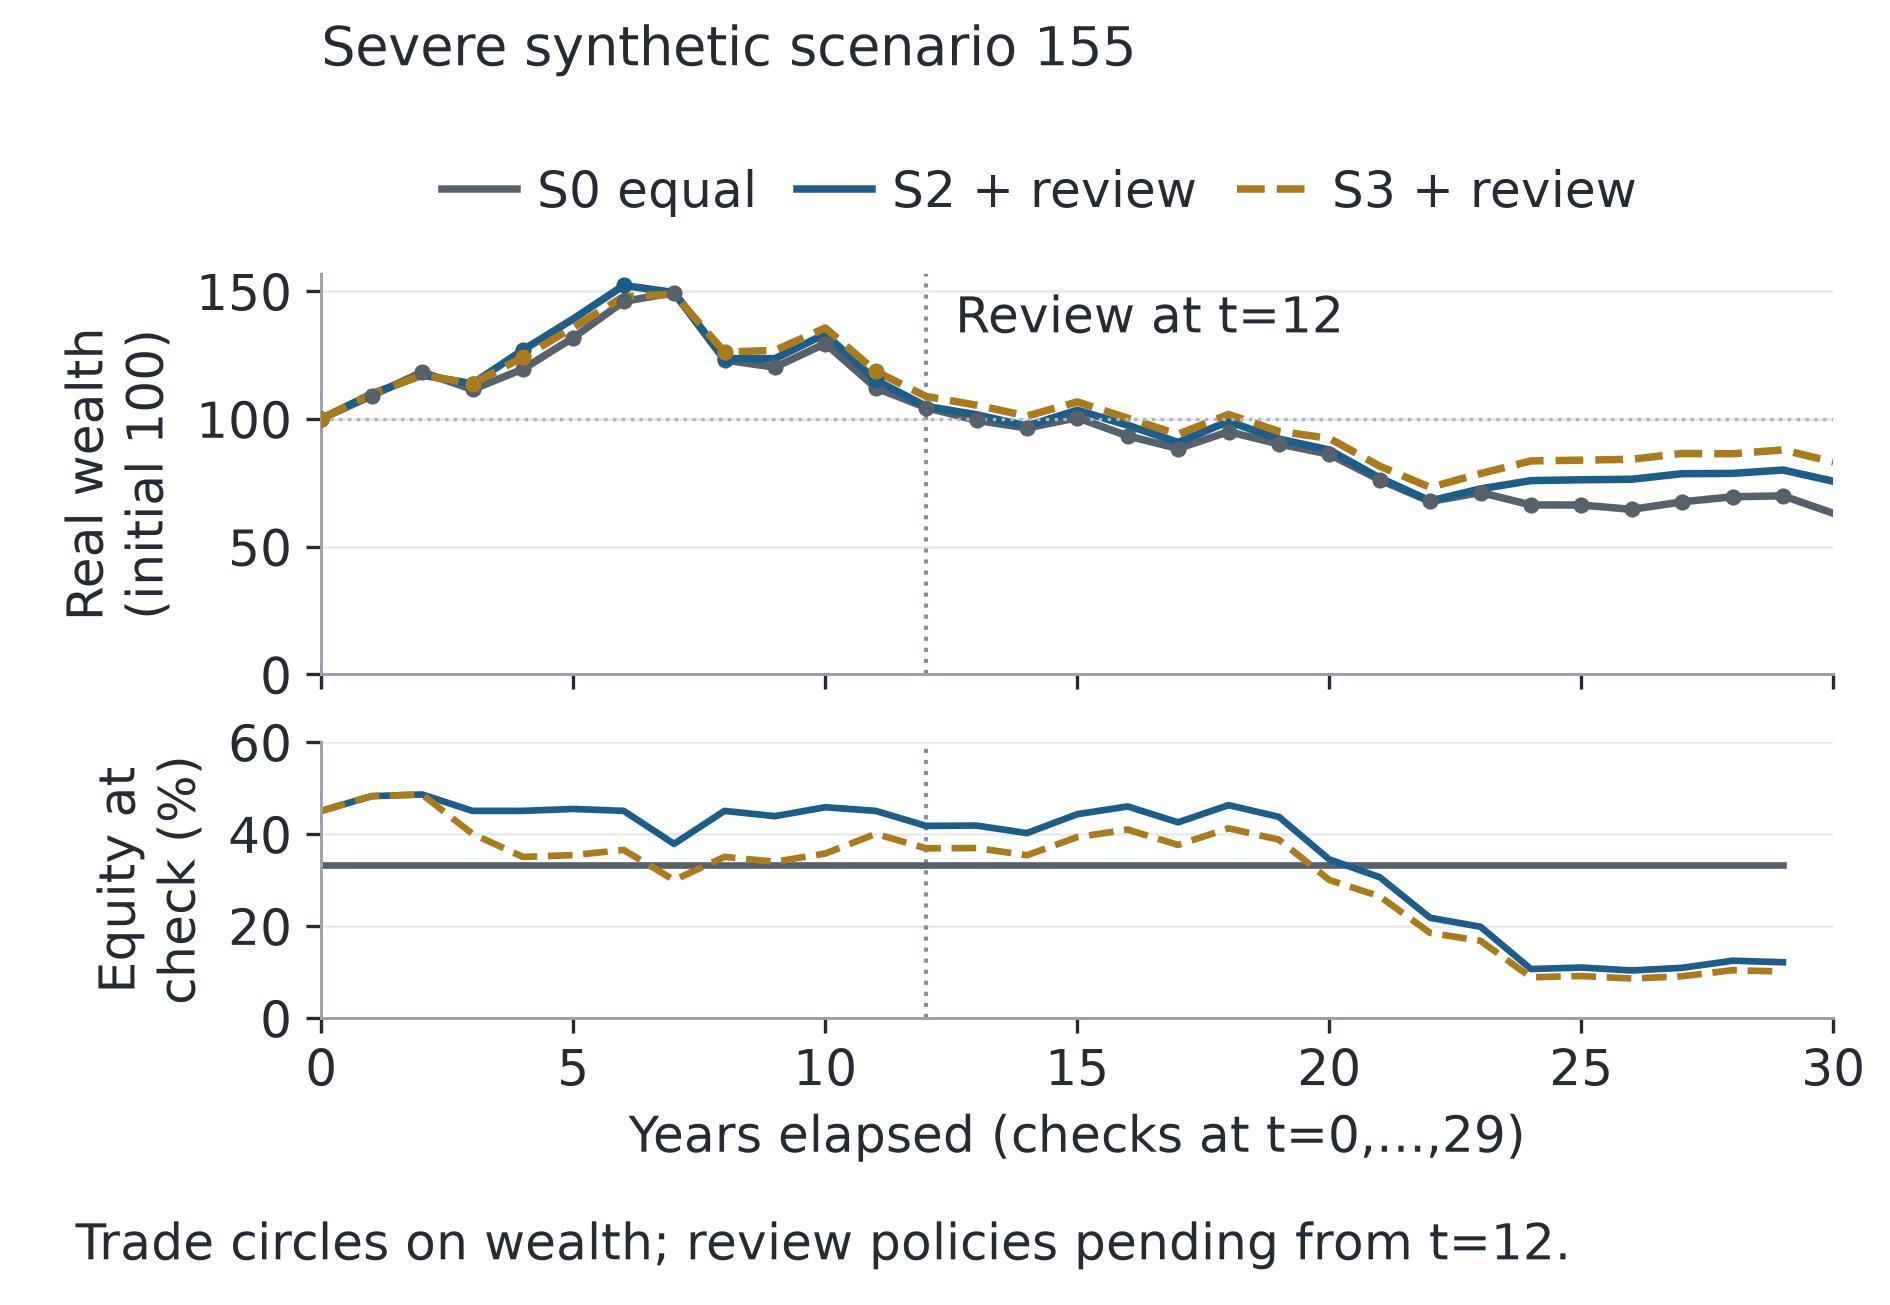
\includegraphics[width=0.94\linewidth]{03_severe_scenario.png}
\caption{Scenario 155: actual purchasing-power wealth and equity exposure.
Decisions for a year precede its returns. Review starts at period 13 after
observing the first 12 years; pending is not a liquidation.}
\end{figure}

\begin{center}\begin{tabular}{lrrr}\toprule
Rule & Real terminal wealth & Maximum drawdown & Trades\\\midrule
S0 & 63.00 & 57.81\% & 30\\
S2 & 58.27 & 62.58\% & 13\\
S2+R & 75.55 & 55.42\% & 6\\
S3+R & 83.11 & 50.83\% & 5\\\bottomrule
\end{tabular}\end{center}
S2+R ends below its original purchasing power despite its higher terminal
wealth than S0 on this path. Its worst drawdown occurs in year 22, after review
begins. A pause therefore does not insure the customer's wealth. Across all
paths, 29/60 enter S2+R review, raising a material human-capacity issue.

The review ablation lowers P90 drawdown from 46.00\% (S2) to 43.44\% (S2+R),
but the paired difference interval is $[-6.75,+1.70]$ percentage points.
Neither this nor its utility interval establishes a general loss-reduction
effect. Its defensible role is halting unsupported automated decisions.

\textbf{Customer-facing message (37 words):}\par
\emph{Your portfolio's purchasing-power loss has reached our review threshold.
We have paused automatic trading and requested an adviser review. Your current
investments remain exposed to market changes; this pause does not guarantee
recovery or prevent further losses.}

\newpage
\section{Reliability, customer calibration and limitations}
We vary transaction costs without refitting weights, forecasts or decision
settings. The chosen rule remains S2+R; only its actual costs and consequently
permitted decisions change.
\begin{table}[H]\centering
\caption{Frozen-rule cost sensitivity, 60 final 30-year scenarios; all entries
other than rule labels are percentages.}
\begin{tabular}{rlrrr}\toprule
Fee rate & Rule & Median $G$ & P90 $D$ & Trade rate\\\midrule
\input table_costs.tex
\bottomrule\end{tabular}
\end{table}
The growth advantage and higher tail drawdown versus equal weights persist
over this range. This supports the same qualified conclusion, not universal
robustness. For a separately recomputed 15-year horizon, S2+R median CAGR is
3.730\%, versus 3.763\% for S0; P90 drawdown is 33.99\% versus 34.10\%.
The 30-year growth advantage cannot be generalized to every customer horizon.

\begin{table}[H]\centering
\caption{Frozen customer assignments audited at their own horizons. These
exceedance rates are empirical, not loss guarantees.}
\begin{tabular}{clrrr}\toprule
Client & Frozen product & Development & Final & Final upper 95\%\\\midrule
B & Conservative, 15 years & 2/120 & 4/60 (6.7\%) & 15.9\%\\
C & Balanced, 30 years & 12/120 & 10/60 (16.7\%) & 28.0\%\\
E & Conservative, 6 years & 0/120 & 0/60 (0.0\%) & 6.0\%\\\bottomrule
\end{tabular}
\end{table}
The upper endpoints are from two-sided 95\% Wilson intervals. C's final point
estimate no longer passes the 10\% screen, although its interval still includes
10\%; this is not statistical proof of a true exceedance rate above 10\%.
It is insufficient evidence for reliable unattended suitability. We preserve
the frozen C assignment to expose this weakness and recommend human confirmation
before deploying it. C's diagnostic review trigger is its own 40\% tolerance,
not the generic experiment's 25\%, so its P90 drawdown (46.00\%) is not the
main-table 43.44\%.

Important limitations are annual observation, synthetic representativeness,
small tail samples, policy-dependent risk preferences and liquidity floors,
and a stationary block forecast. Overlapping blocks do not create additional
independent evaluation scenarios. Real customers' income, reserves and
withdrawal timing are absent. Pending behaviour is mechanical; no evidence
about an adviser's actual intervention benefit is available.

\newpage
\section{Recommendation and reproducibility}
Use the 15/5/80 Conservative, 45/10/45 Balanced and 90/5/5 Growth targets as
an explicit catalogue for this study. Refer A and D; assign B and E to
Conservative. The frozen rule assigns C to Balanced, but the
borderline development screen does not retain its pointwise calibration in
final data: require human confirmation before unattended use. Growth need not
be assigned to any of these five profiles. Questionnaire tolerance is not a
promise to cap losses.

For Balanced, retain fixed targets with cost-aware execution and an explicit
review state. Do not enable automatic target updates on the current evidence.
The proposed rule trades less and has higher 30-year median growth than the
required benchmark, but its tail drawdown is higher and the utility advantage
is uncertain. The main safeguard is suspension of unsupported automatic
decisions with clear customer communication; holding during review can still
lose money and needs practical human-response capacity.

The supplementary archive contains source code, input attribution, fixed
protocol, model fingerprints, per-scenario paths, all reported tables, figure
builders, report source and an independent result audit. Financial identities,
future-information perturbations, target bounds and review-state tests are
automated. Reproduction stages are \texttt{develop}, \texttt{freeze} and
\texttt{final}; existing frozen/final archives cannot be silently overwritten.
The public repository is \url{https://github.com/Lebmar/GKG-MCM}.

\section*{References}
\begin{enumerate}[label={[\arabic*]},itemsep=4pt]
\item HKUST(GZ) MCM organisers (2026). \emph{Senior Group Problem A:
SafeInvest}, supplied statement and synthetic dataset. CC BY-NC-SA 4.0.
\item Jord\`a, \`O., Schularick, M., and Taylor, A. M. (2017).
Macrofinancial History and the New Business Cycle Facts. \emph{NBER
Macroeconomics Annual}, 31. Database: \url{https://www.macrohistory.net/database/}.
\item Jord\`a, \`O., Knoll, K., Kuvshinov, D., Schularick, M., and Taylor,
A. M. (2019). The Rate of Return on Everything, 1870--2015.
\emph{QJE}, 134(3), 1225--1298. doi:10.1093/qje/qjz012.
\item Boyd, S., et al. (2017). Multi-Period Trading via Convex Optimization.
\emph{Foundations and Trends in Optimization}, 3(1), 1--76.
doi:10.1561/2400000023.
\item DeMiguel, V., Garlappi, L., and Uppal, R. (2009). Optimal Versus Naive
Diversification: How Inefficient is the 1/N Portfolio Strategy?
\emph{RFS}, 22(5), 1915--1953. doi:10.1093/rfs/hhm075.
\item Magdon-Ismail, M., Atiya, A. F., Pratap, A., and Abu-Mostafa, Y. S.
(2004). On the Maximum Drawdown of a Brownian Motion.
\emph{J. Applied Probability}, 41(1), 147--161.
\url{https://doi.org/10.1239/jap/1077134674}.
\end{enumerate}

\section*{Use of AI Tools}
OpenAI Codex assisted with problem interpretation, model design, Python code,
independent AI review, experimental analysis and English drafting. Automated
tests and independent numerical checks were used to verify accounting,
causal timing and reported calculations; bibliographic records were checked
against primary sources. These checks do not replace the author's review.
The author remains responsible for correctness, attribution and the submission.
\end{document}
